
\chapter{Applikasjon}

I dette kapittelet vil det bli gjort rede for utviklingen og de applikasjonen.


\section{Utvikling}


Målet med forskningen er å undersøke potensielle forbedringer funksjonene beskrevet i seksjon \ref{sec:ResearchQuestion} kan ha på den eksisterende løsningen Tobii Sono Flex (\ref{chap:Tobii-Sono-Flex}). Det mest naturlige valget for å implementere disse funksjonene ville vært å ta utgangspunkt i den eksisterende kildekode og utvidet med nødvendig kode. Problemet var at plattformen som den eksisterende koden var bygget på hadde flere begrensninger og ville gjort det vanskelig å fått implementert mye av funksjonalitet som skulle undersøkes, spesielt gjelder det animasjonene. Dette gjorde at utviklingen ble startet som et nytt prosjekt og at første del av utviklingen var å lage en forenklet prototype av den samme applikasjonen bare på en annet rammeverk.

\subsection{Rammeverk}

Siden grunnen til at utviklingen begynte med blanke ark var begrensninger i det eksisterende rammeverket, var det viktig at den nye som applikasjonen skulle bygges på, ikke hadde dem. Valget ble derfor basert på at den var tilrettelagt for implementering av ønsket funksjonalitet. Det vil si god støtte for brukergrensesnitteknologi som animasjon, lyd og bildebruk. En annen viktig faktor var at rammeverket måtte være kompatibelt med øyestyringsenheten Tobii PCEye GO.
Valget falt derfor på Microsoft .NET. Grunnen til dette var at rammeverket oppfylte alle kravene og er godt dokumentert.


Arkitekturen til .NET er omfattende og som en kan se utifra figur \ref{fig:net-arkitektur} er det flere programmeringspråk og komponenter en kan velge å ta i bruk. Rapporten vil derimot kun gi informasjon om de ulike komponentene fra .NET som ble brukt og er nødvendig for videre lesning.


\begin{figure}[ht]
\centering
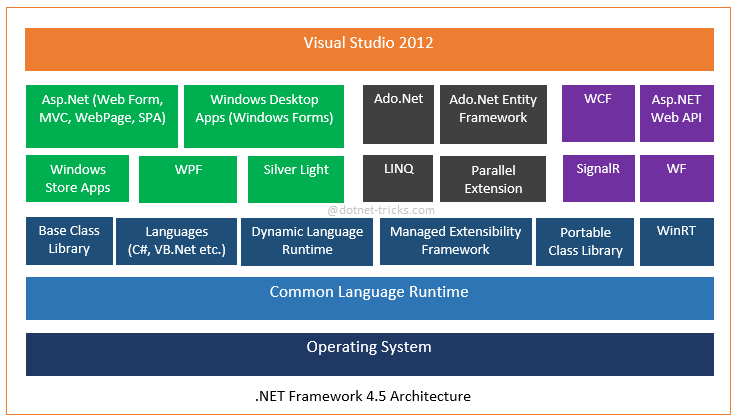
\includegraphics[width=140mm]{netframework45}
\caption{Diagram som viser arkitekturen til .net rammeverket versjon 4.5}
\label{fig:net-arkitektur}
\end{figure}

\subsection{Windows Presentation Foundation}

Det er hovedsaklig to delsett av .NET som er brukt til å utvikle applikasjonen, programmeringspråket C-sharp sammen med presentasjonssystemet Windows Presentation Foundation (\gls{WPF}).  WPF er et grafisk system for å lage brukergrensesnitt og tilhørende logikk til Windows-baserte applikasjoner som utnytter den grafiske maskinvaren best mulig. WPF bruker eXtensible Application Markup Language (\gls{XAML}), som er et XML-basert språk til å definere og kombinere ulike grensesnittelementer. Figur \ref{lst:myLabel} viser hvordan et vindu med en knapp er definert i XAML. Resultatet kan ses i figur \ref{fig:xamlButton}. 

\begin{lstlisting}[language=java,caption={Kodesnutt skrevet i XAML som viser en enkel applikasjon med en knapp}
\label{lst:myLabel}, belowcaptionskip=4pt]
<Window xmlns="http://schemas.microsoft.com/winfx/2006/xaml/presentation" Title="Window with Button"  Width="250" Height="100">

  <Button Name="button" Click="button_Click">Click Me!</Button>
  
</Window>
\end{lstlisting}

\begin{figure}[ht!]
\centering
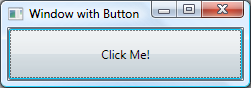
\includegraphics[width=100mm]{xamlButton}
\caption{Skjermdump av det applikasjonen som blir gjengitt ved kjøring av kodefnutt \ref{lst:myLabel}}
\label{fig:xamlButton}
\end{figure}


For å kunne samhandle med de grafiske objektene definert i XAML filen opprettes det alltid en tilhørende kodefil sammen med denne. Kodefilens formål er å ta seg av data og logikk for å ha et klart skille mellom utseende-spesifikk kode og oppførsel-spesifikk kode. For eksempel så vil en knapp sitt utseende og plassering bli definert XAML filen, mens hvordan data blir påvirket av interaksjon med knappen blir definert i den tilhørende kodefilen.



Den tilhørende kode-filen til XAML koden beskrevet i kodesnutt \ref{lst:myLabel} er vist i kodesnutt \ref{lst:backbutton}. Ved å trykke på knappen bildet vil metoden button\textunderscore Click i kodefilen bli kalt og en dialogboks vist til brukeren.

En XAML fil definerer som tidligere nevnt grafiske objekter som vindu, side eller brukerkontroll, men for at en bruker skal kunne samhandle med applikasjonen trengs de


Vindu inneholder er en konteiner som inneholder alle applikasjonens grafiske elementer. En

For å håndtere logikken og interaksjon med brukergrensesnittet,  definert i XAML, brukes det en kodefil. For hver XAML   Dette Dette gjør at koden har et klart skille mellom utseende-spesifikk kode og oppførsel-spesifikk kode.

Som tidligere nevnt defineres brukergrensesnittet i XAML,

WPF oppfordrer til å skille mellom utseende spesifikk kode og oppførsel-spesifikk kode ved at grafiske elementer skrives i XAML og interaksjonen  kun brukes til generere 
XAML brukes til å generere brukergrensesnitt, 
Hver XAML-fil har en tilhørende kode-fil for håndtering av hendelser og oppførsel. Dette gjør at koden har et klart skille mellom utseende-spesifikk kode og oppførsel-spesifikk kode. Den tilhørende kode-filen til XAML koden beskrevet i kodesnutt \ref{lst:myLabel} er vist i kodesnutt \ref{lst:backbutton}. Ved å trykke på knappen bildet vil metoden button\textunderscore Click i kodefilen bli kalt og en dialogboks vist til brukeren.

\begin{lstlisting}[language=java,caption={falafel}
\label{lst:backbutton}]
 void button_Click(object sender, RoutedEventArgs e)
        {
         Viser en dialogboks naar knappen trykkes
        MessageBox.Show("Hallo!");
        }
\end{lstlisting}



\section{Layou}

Prototypen har den samme layouten som Tobii Sono Flex, med en menylinje etterfulgt av en symboltabell under. 


\section{Animasjon}

Animasjoner i programvare brukes som et virkemiddel for å tiltrekke seg oppmerksomhet, underholde eller demonstrere noe. Det kan enten være en kort animasjon der en knapp tiltrer til en side når man svever over den med musen eller det kan være av den lengre sorten som en flash-video.  Animasjon er i hovedsak alt som beveger seg i applikasjonen. Selv om dynamikken som animasjoner kan fungere som et positivt virkemiddel viser undersøkelser gjort av Nielsen og Loranger \cite{NielsenBok}  at for mye blinkende og bevegende elementer kan slite ut brukeren og gjør det vanskeligere å fokusere på oppgaven. Med animasjonene som er implementer ønsker vi å undersøke dette. Hvilke animasjoner fungerer som et hjelpemiddel og med det gir verdi til applikasjonen og hvilke som er distraherende for brukeren og gir en uønsket effekt.

I denne prototypen skjer animasjonene som en respons på at brukeren trykker på et symbol. Hva som skjer avhenger av hvilken type symbol det er. De ulike typene som finnes i symboltabellen ble forklart i seksjon \ref{subsubsec:symboltabell}, og er ordsymbol, kategorisymbol og navigasjonssymbol.


\subsection{Animasjoner: ordsymbol}

Når en bruker trykker på et ordsymbol, vil symbolet legge seg i setningslisten og er da klar for gjøres om til tydelig tale. Når brukeren har fullført setningen i Sono Flex blir brukeren presentert for endringen ved at symbolet vises i setningsfeltet. Med prototypen ønsker vi  å gi en mer visuell representasjon av denne endringen til brukeren. Ved å la brukeren kunne velge mellom to animasjoner som oppstår når han trykker på ønsket ordsymbol. De to animasjonene fungerer som følgende:


I) Brukeren trykker på et ordsymbol.
   Ordsymbolet krympes til 5 prosent av størrelsen.
   I setningslisten vil en kopi av det krympede ordsymbolet dukke opp.
   Kopien forstørres så til den opprinnelige størrelsen.
   Ordsymbolet som opprinnelige ble trykket blir forstørret til opprinnelig størrelse.

   
II) Brukeren trykker på et ordsymbol.
    Ordsymbolet beveger seg ut av sin posisjon og glir mot den posisjonen den vil ha i setningslisten.
    Når den har truffet posisjonen i setninglisten, stopper den opp og blir værende i ro.

    Med disse animasjonen vil en først og fremst gi brukeren beskjed om at et valg har blitt gjort, men de ønsker også gjøre bruk av programvaren mer spennende.  I Sono Flex  vil ingen av knappene ha noe visuelt som gjør at brukeren kan skille hva som skjer, utenom at symboltabellen bytter ut de eksisterende symbolene. I dette tilfelle vil en se at symbolet går fra å være en statisk symbol til å bli flyttet til setningslisten og bli en del av ønsket setning. 



\subsection{Animasjon: Kategorisymbol}

Når en bruker trykker på et kategorisymbol vil symbolene i symboltabellen byttes ut med symbolene som hører til i den gjeldene kategorien. Hvis en trykker på kategorien "dyr" så vil tabellen fylles med ordsymbol som "Hund", "katt", "tiger" o.s.v. Her ønsker animasjonen å hjelpe til med å fortelle at man ikke trykker på ordet dyr, men kategorien dyr og at brukeren får en forståelse for forskjellen mellom dem. Animasjonen startet ved at symbolet som brukeren trykket på forstørres helt til den dekker hele symboltabellen. Det vil si at ingen av de andre symbolene vises, kun kategorisymbolet. Symbolet vil så igjen forminskes, men symbolene i tabellen vil være erstattet av symbolene som tilhører kategorien. 


\subsection{Animasjon: Navigasjonssymbol}


Den siste typen symbol er navigasjon og ved interaksjon vil den navigere mellom sider når det ikke er plass til alle symbolene på en side. Det vil si at symbolet skal kunne navigere fremover, fra side 1 til 2 og 2 til 3 og bakover igjen. Når brukeren trykker fremover starter animasjonen ved at alle symbolene som er på gjeldene side og neste side begynner å bevege seg mot venstre. Slik at symbolene på gjeldene side kontinuerlig blir byttet ut med de på neste. Symbolene på siden sklir ut, mens symbolene på neste sklir inn og overtar plassene. Når brukeren nå trykker på bakover-symbolet vil det samme skje bare at symbolene sklir mot høyre.



\section{Lydeffekter}

Som en del av rapporten ønsket vi å undersøke hvilken påvirkning lydeffekter hadde på brukeren. Hovedsaklig var målet å finne ut to ting. I hvilken grad hjelper effektene brukeren i å navigere rundt i applikasjonen og om det vil påvirke brukerens helhets uttrykk av applikasjonen. 

\subsection{Lydeffekter i prototypen}

I prototypen er effektene brukt for å gi brukeren tilbakemelding på et valg han har foretatt seg, har blitt registrert av programvaren. 



I prototypen er det lagt til flere lydeffekter, utelukkende i form av små lydklipp på maks 1 sekund. Effektene vil kun bli avspilt som en respons til noe brukeren foretar seg eller som å informere om en hendelse. Denne begrensning finnes for å ikke skape forvirring hos brukeren. Hvis lyd også hadde blitt avspilt tilfeldig så ville meningen med effektene forsvinne. Fordi brukeren blir lurt til å tro at programvaren har registrert en interaksjon, selv om han ikke har foretatt seg noe. Det er derfor viktig at det er lett for brukeren å skille mellom effektene som representerer en interaksjon og informasjon. De ulike interaksjonslydeffektene er også forskjellige, og hvilken som blir spilt er avhengig av,  som med animasjo,  hvilken type komponent brukeren samhandler med. 





Dette vil forhåpentligvis gjøre at brukeren mer effektivt kan bekrefte valget og fortsette med oppgaven. Som 




Hvilken brukeren blir presentert for er avhengig av hvilket komponent han interagerer med.  Grunnen er at hvis effektene hadde blit avspilt uten at brukeren foretar seg noe, så kan


Hvilken lyd som blir avspilt er avhengig av hvilket valg brukeren har foretatt seg, og responsen til brukeren vil 

Eksmepelvis hvis brukeren foretar seg et ulovlig valg vil han bli presentert for en lyd som har gir negative assosiasjoner.  D

Lyden som vil bli gitt til brukeren vil komme i form av små lydklipp som maks vil vare i et sekund,  ettersom det skal være nok for at brukeren kan registrere det. 

 Tilbakemelding i form av lyd gir brukeren en bekreftelse på at han valget han nettopp har foretatt har blitt registrert og 







Ta for eksempel brødristeren. Når den er ferdig vil brødet hoppe opp, men i tilegg vil den gi fra seg et pling. Altså brukeren vil få tilbakemelding på at han kan hente brødet både visuelt(brødet som hopper opp) og gjennom lyd(plinget). Ved å g

Lyd brukes ofte for å fortelle brukeren av produktet noe. For eksempel vil brødristen gi fra seg et pling når den er ferdig samtidig med at skivene hopper opp av maskinen. I dette tilfellet vil 


I dag brukes lyd ofte i flere sammenhenger, i alt fra